\documentclass[10pt,a4paper]{ULBreport}
\usepackage[utf8]{inputenc}
\sceau{pic/official_logos/sceauULB.png}
\graphicspath{ {./pic/} }
\usepackage{multirow}
\usepackage{listings}
\usepackage{color} 
\usepackage{setspace} 
\usepackage{amsmath}
\usepackage{hyperref}
\usepackage{pdfpages}
\usepackage{biblatex}
\usepackage{floatrow}
\usepackage{subcaption} 
\usepackage{siunitx}
\usepackage[many]{tcolorbox}
\usepackage{multirow}
\usepackage{listings}
\usepackage[dvipsnames]{xcolor}
\usepackage{fancyvrb}

\usepackage{xstring}
\usepackage{etoolbox}

% Colors



\begin{document} 


	\titleULB{
	title={DVB-C project},
    studies={M1-IRELE},
    course ={ELEC-H401 Modulation and coding},
    author={\textit{Authors :} \\ Arico Amaury \\ Colot Emmeran },
    date={\textbf{Academic year :} \\ 2024 - 2025},
    teacher={\textit{Professor : } \\ Horlin François},
    logo={pic/official_logos/logos.jpg},
    manyAuthor
	}

%\listoftables % ToC for tables

%\listoffigures % ToC for figures

\setcounter{secnumdepth}{-1}

\chapter{Introduction}

This report aims to complete the code that simulates a DVB-C transmission chain in matlab. It answers the questions asked after each major step of the project and analyses the results of the simulation.

\vspace{2cm}

\begin{figure}[H]
    \centering
    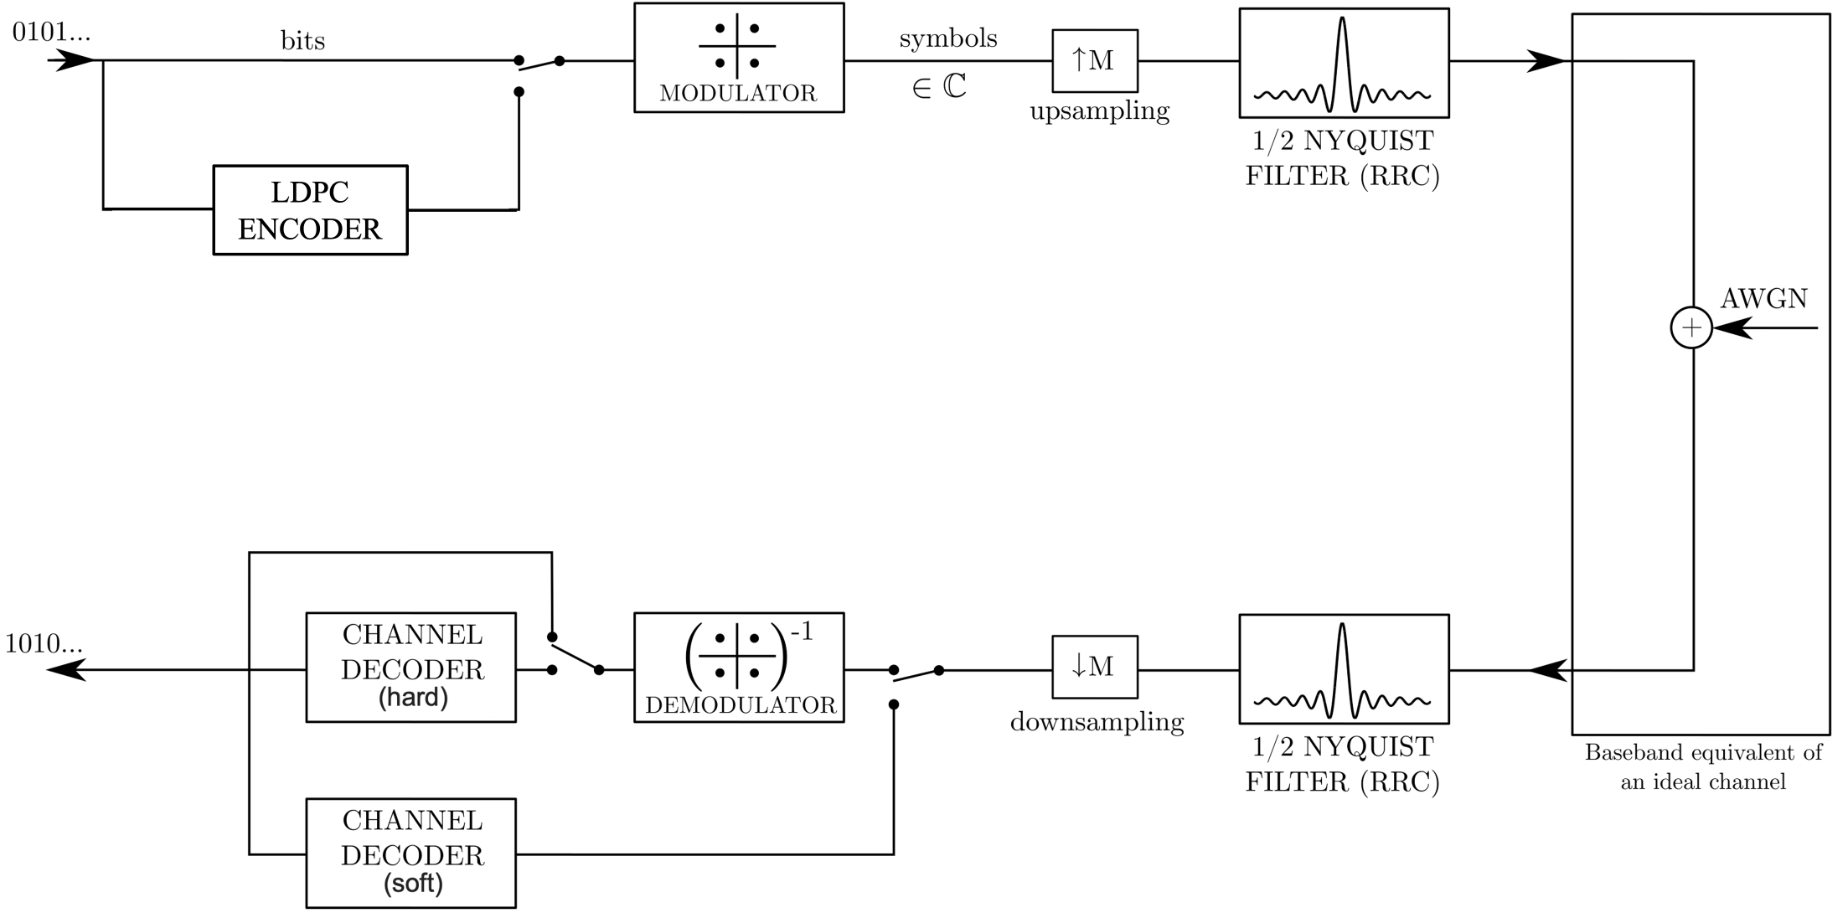
\includegraphics[width=0.9\linewidth]{blockDiagram.png}
    \caption{DVB-C transmission chain}
    \label{fig:blockDiagram}
\end{figure}

\setcounter{secnumdepth}{-1}

\chapter{Transmission chain blocks}

\section{Baseband representation}

By looking at the block diagram of the transmission chain \ref{fig:blockDiagram}, one can see we never move the baseband signal to the carrier frequency. As the simulation runs on a computer, using the bandpass representation of the signal would require much more samples as the sampling frequency would need to be at least twice the carrier frequency. By simulating the chain in baseband, the minimal sampling frequency is reduced to the symbol rate in order to have at least one sample per symbol. \\
Because the signal is oversampled, the sampling frequency is then equal to the symbol rate multiplied by the oversampling factor. \\

\section{Modulation and Demodulation}

After generating N random bits, they are modulated. This allows to send fewer symbols than the number of bits. We chose QAM modulation as it combines ASK and PSK. Depending on the number of bits per symbol ($N_{\text{bps}}$), the number of bits sent ($N$) had to be chosen such that  $N / N_{\text{bps}} \in \mathbb{N}$. \\
Figure \ref{fig:QAMComparison} compares the modulation the constellation diagrams obtained for QAM-16 and QAM-64. As the constellations points are more spaced on the left, QAM-16 is less prone to a wrong demodulation (when noise will be added). This comes at the cost of a lower bitrate: for the same symbol rate, QAM-64 will send 6 bits while QAM-16 only send 4. It clearly shows a compromise between reliability and capacity. \\

\begin{figure}[H]
    \centering
    \begin{subfigure}[b]{0.45\linewidth}
        \centering
        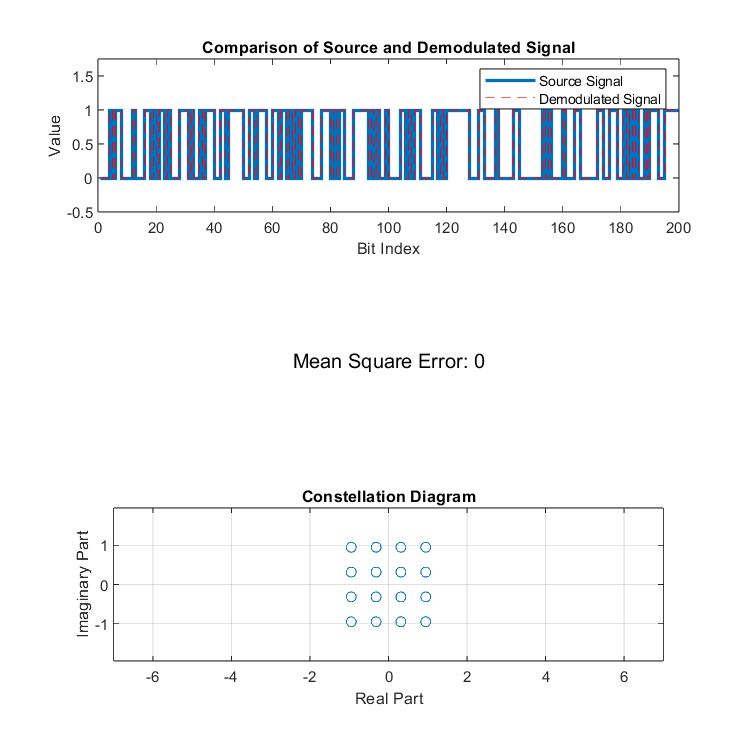
\includegraphics[width=\linewidth]{modulation16.png}
        \caption{QAM-16 modulation}
        \label{fig:QAM16}
    \end{subfigure}
    \hfill
    \begin{subfigure}[b]{0.45\linewidth}
        \centering
        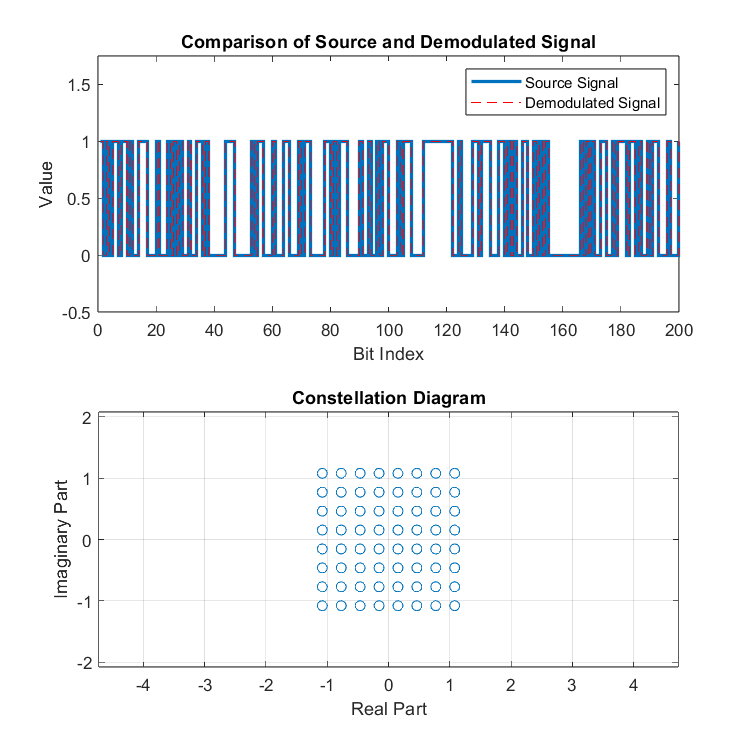
\includegraphics[width=\linewidth]{modulation64.png}
        \caption{QAM-64 modulation}
        \label{fig:QAM64}
    \end{subfigure}
    \caption{Comparison of QAM modulations, where the mean square error is computed between the transmitted and received bitstream}
    \label{fig:QAMComparison}
\end{figure}

\section{Optimal demodulator and detector}

First, it is important to remind that the transmitted signal is characterised / represented by a set of coefficients which results from the projection
 of the signal on the adequate orthonormal basis function related to the choosen modulation.
 Once transmitted, the signal is affected by noise (in our case AWGN noise).  In the general case, this noise reoriante the signal representation outside of the sub-space set during the modulation phase.
To construct an optimal demodulator, 2 criteria should be taken into account.  The first one is the sufficient statistic criteria.  It is proven that once the received signal
is projected on the sub-space defined by the previous basis functions, the noise component outside of the sub-space is indepedent from the projected signal.
It means that we loose no information by projecting the received signal on the original sub-space and we can therefore make an optimal decision based on projected signal.
(based on the coefficient of the projected received signal).

\begin{figure}[H]
    \centering
    \includegraphics[scale = 0.7]{Bank_correlator.png}
    \caption{Projection on basis sub-space}
    \label{fig:Bank_correlator}
\end{figure}

\begin{figure}[H]
    \centering
    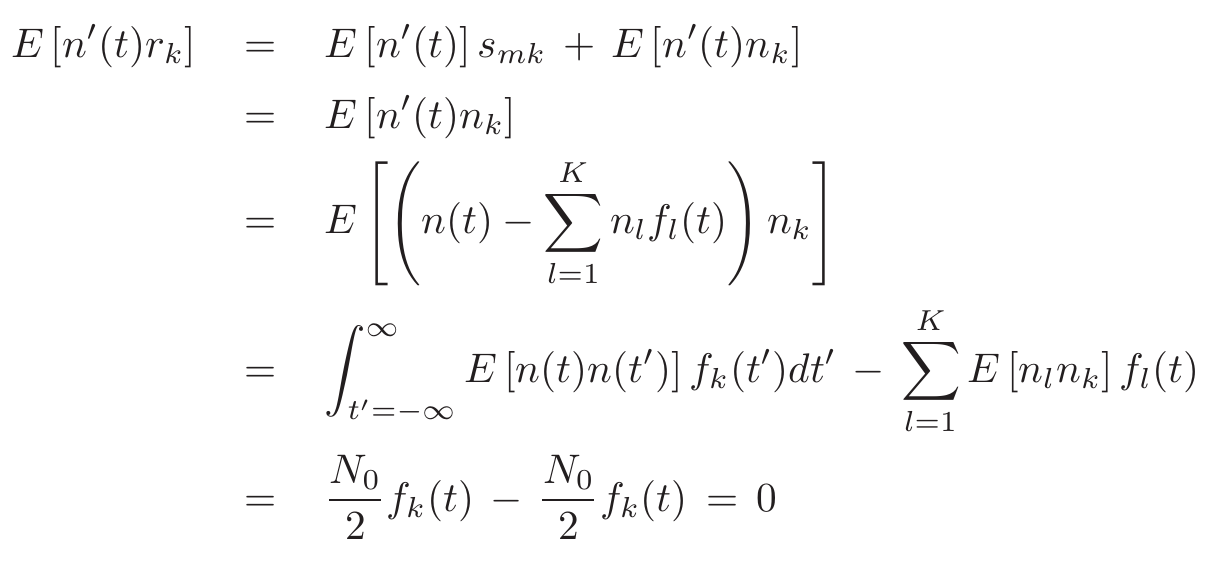
\includegraphics[scale = 0.5]{SufficientStatistic.png}
    \caption{Criteria of sufficient statistics}
    \label{fig:Sufficientstatistic}
\end{figure}

The second criteria is the usage of matched filters. The demodulator used to achieve the sufficient statistic property is composed of bank of correlators (projection of basis function).
Instead of using a bank of correlator, we can use a bank of filters matched to the used basis functions.  It is proven that such filters at the demodulator results to
 a maximized SNR (minimize the power of the noise at the exit of the demodulator).
In conclusion, by using a bank of filters matched on the orthonormal basis function set by the choice of the modulation, we cna construct a optimal demodulator which
 would ensure an optimal decision based on the received signal and ensure a maximum SNR at the output of this demodulator.

 \begin{figure}[H]
    \centering
    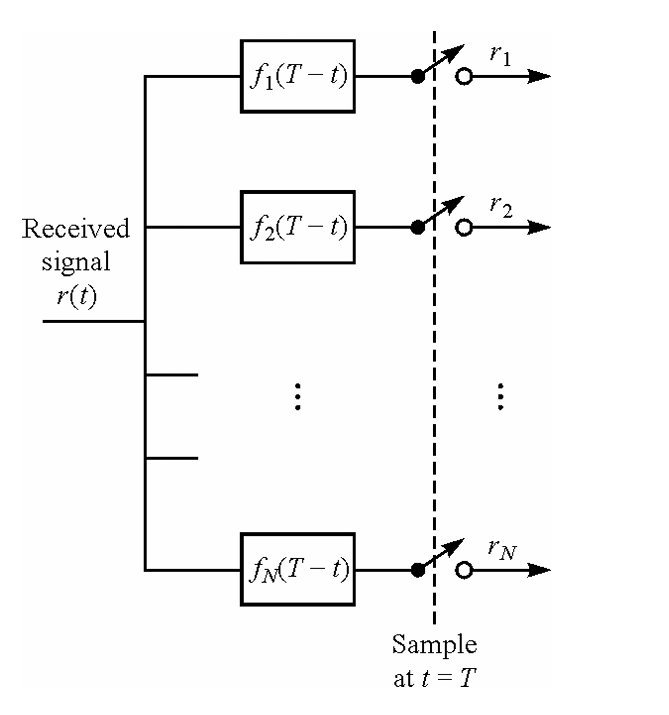
\includegraphics[scale = 0.6]{Matchedfilters.png}
    \caption{Bank of filters matching basis functions}
    \label{fig:Matchedfilters}
\end{figure}

\begin{figure}[H]
    \centering
    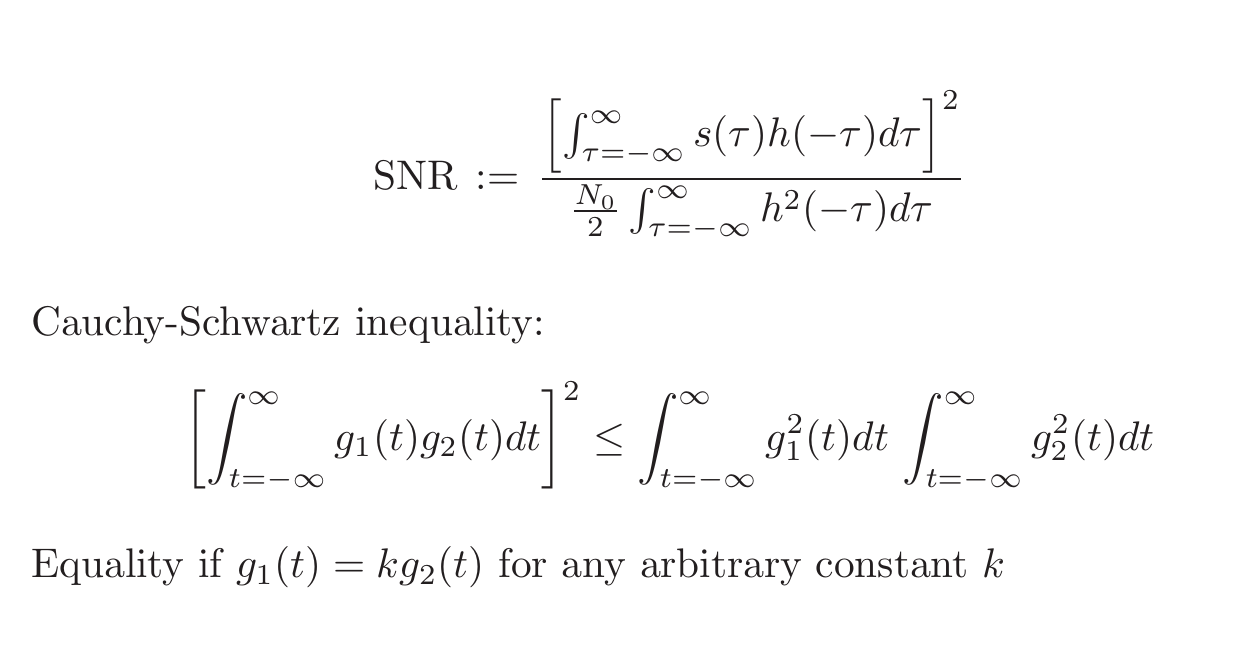
\includegraphics[scale = 0.5]{MaxSNR.png}
    \caption{Maximum SNR demonstration}
    \label{fig:MaxSNR}
\end{figure}

At the output of the demodulator, we still need to ensure to make the optimal choice of the M possible sm(t) based on the received signal.
For that, we would need to follow the maximum likelihood criteria which refers from the maximum a posteriori criteria (general criteria) if each possible sm(t) 
owns the same probability.
The criteria leads to the following result : the optimizal sm(t) choice is found by taking the minimum euclidian distance between the observable received signal r(t) 
and all the possible modulated signal sm(t).

\section{Pulse shaping}

With modulation only, the bandwidth of the transmitted signal is infinite. This is problematic as it could interfere with neighboring channels. A filtering is applied to resolve this but the chosen filter must respect two other constraints: it must cancel inter-symbol interference (ISI) and must maximize the SNR. \\
The raised cosine filter is chosen as it limits the bandwidth and cancels ISI. To maximize the SNR, it is applied as a matched filter by using the square root of it at the transmitter and at the receiver. \\
The time domain and frequency domain representation of the raised cosine filter is shown in Figure \ref{fig:raisedCosine}. Figure \ref{fig:pulseShaping} shows how the signal is shaped in the time domain and how there is indeed no ISI. Finally, the spectrum of the transmitted signal is plotted in figure \ref{fig:shapedSpectrum} where the frequency band is limited to $[-3, 3]$MHz. \\

\begin{figure}[H]
    \centering
    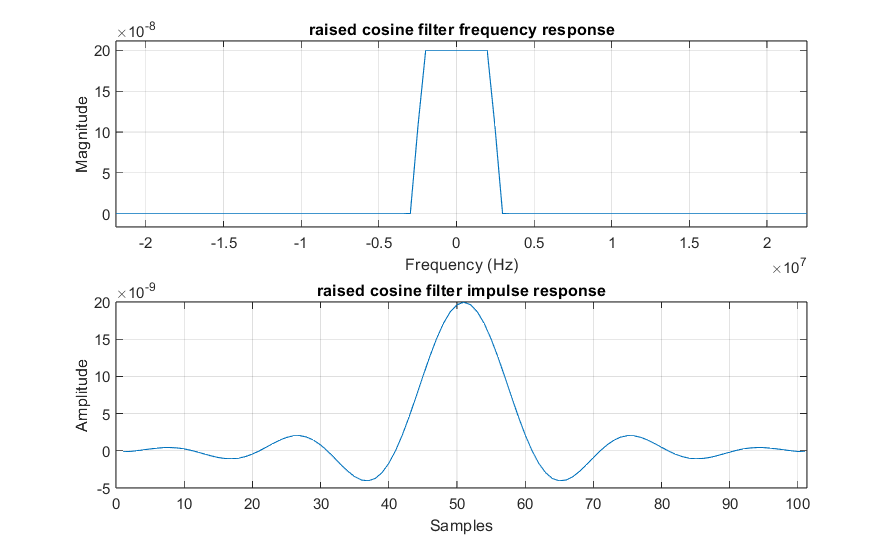
\includegraphics[width=0.9\linewidth]{raisedCosine.png}
    \caption{Time and frequency domain representation of the raised cosine filter}
    \label{fig:raisedCosine}
\end{figure}

\begin{figure}[H]
    \centering
    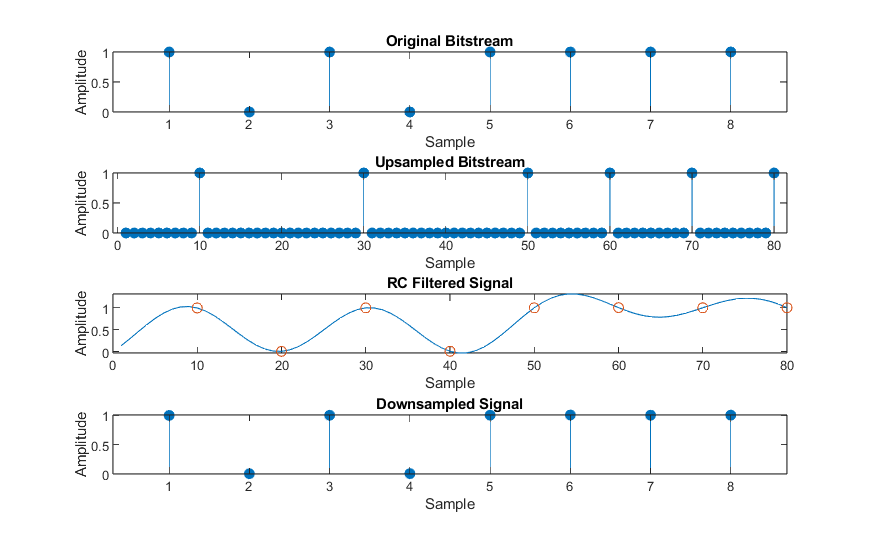
\includegraphics[width=0.9\linewidth]{pulseShaping.png}
    \caption{Pulse shaping with a raised cosine filter}
    \label{fig:pulseShaping}
\end{figure}

\begin{figure}[H]
    \centering
    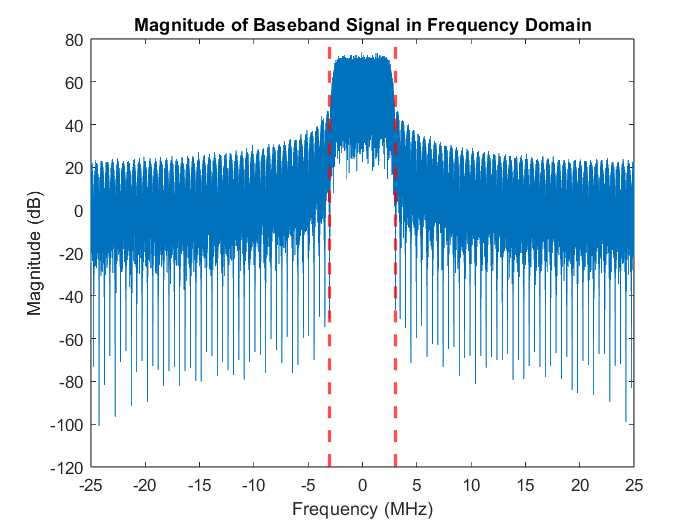
\includegraphics[width=0.9\linewidth]{shapedSpectrum.png}
    \caption{Spectrum of the transmitted signal after pulse shaping}
    \label{fig:shapedSpectrum}
\end{figure}

\section{Noise addition}

The last building block is a noise source. It generates additive white Gaussian noise in baseband. When the signal is corrupted too much, the demodulation can fail. The BER curves are plotted in figure \ref{fig:BER} and they show the impact of the noise power $N_0$ on the bit error rate. The compromise between reliability and capacity is again visible: in the same conditions (same $E_b/N_0$), a modulation with lower capacity will have a smaller BER. \\

The theoretical BER curves are plotted on figure \ref{fig:BER} and are compared with the simulation results. They stay close to each other untill the BER reaches $10^{-4}$. This limit could go even lower by increasing the number of bits sent but we limited it to $10^6$ in order for the code to run quite fast. \\

To impose a value of $E_b/N_0$, we start by computing the energy of the transmitted signal before adding the noise. The power of the noise is then chosen as $N_0 = E_b / (E_b/N_0)_{\text{desired}}$. \\

\begin{figure}[H]
    \centering
    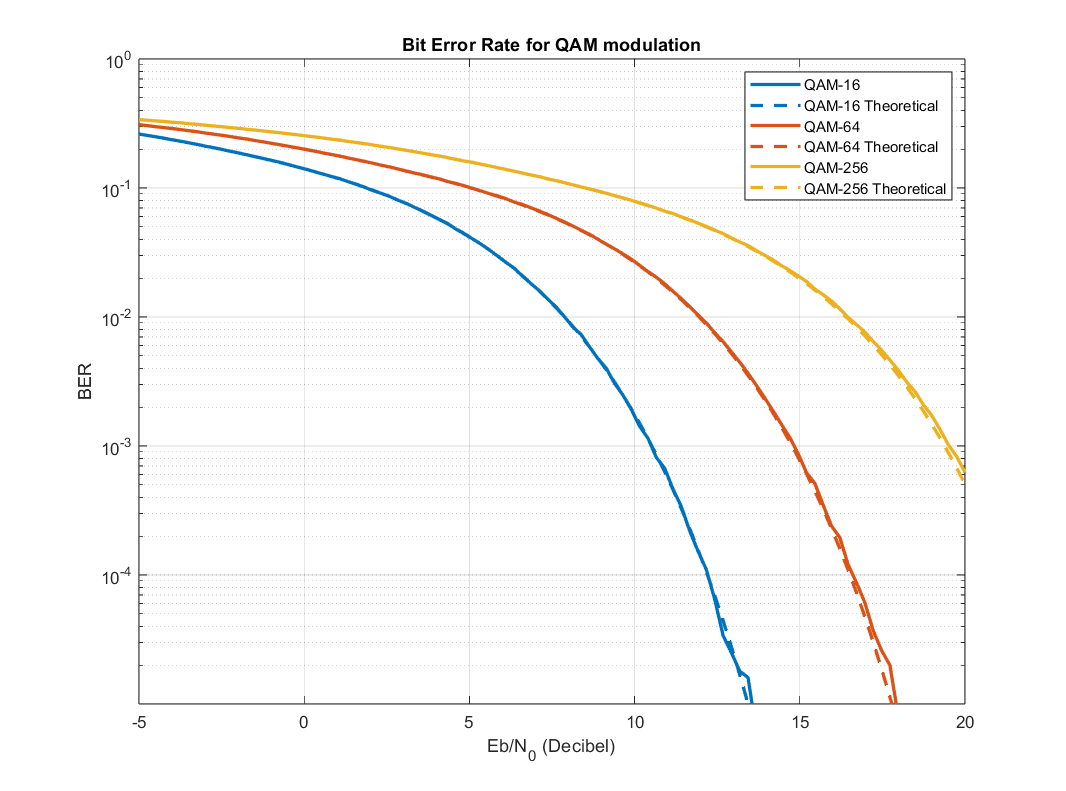
\includegraphics[width=0.9\linewidth]{BERcurve.png}
    \caption{BER curves for different QAM modulations}
    \label{fig:BER}
\end{figure}

\section{Bit rate}

Considering the following characteristics :

    \begin{itemize}
        \item (a) Physical bandwidth of 6 MHz
        \item (b) Roll-off factor = 0.2 
        \item (c) QAM 16 modulation 
    \end{itemize}

We can derive the symbol rate from the physical bandwidth

\begin{equation*}
    f_{symbol} = \frac{B_{physical}}{roll-off-factor} = 5 MHz
\end{equation*}

\begin{equation*}
    Bit-rate = Symbol-rate * Bits-per-symbol = 5MHz*4 = 20 MBps
\end{equation*}


\setcounter{secnumdepth}{-1}

\chapter{Synchronization errors}

\section{Description}

Because the receiver and transmitter are not at the same location, the carrier frequencies and the samplers at TX and RX will have a different phase and due to the inaccuracies of the oscillator, the frequencies will also be slightly different. \\
This is summarized in 4 effects:
\begin{itemize}
    \item \textbf{Carrier frequency offset (CFO)}: The difference in the carrier frequencies at TX and RX ($=\Delta \omega$). It will add ISI as the RRC are not anymore matched and a linearly increasing phase shift will appear.
    \item \textbf{Phase offset}: The difference between the phase of the carrier signal at TX and RX.
    \item \textbf{Sampling frequency offset (SFO)}: The difference in the sampling frequencies at TX and RX.
    \item \textbf{Time shift}: The difference in the timing of the samples at TX and RX.
\end{itemize}

\section{Implementation}

\subsection{CFO}
The CFO implementation is done by multiplying the signal with a complex exponential $e^{j2\pi \phi_{\text{ppm}}f_c t}$. The phase offset is added to the CFO. It is defined in ppm (part per million) where the ppm value is $\frac{\Delta\omega}{f_c} 10^{-6}$. \\
Figure \ref{fig:CFO_BER} shows the BER curves with different CFO values. In order to have useful results, the linear phase shift is removed right after the second RRC filter. This allows to only keep the effect of ISI on the BER curve.

\begin{figure}[H]
    \centering
    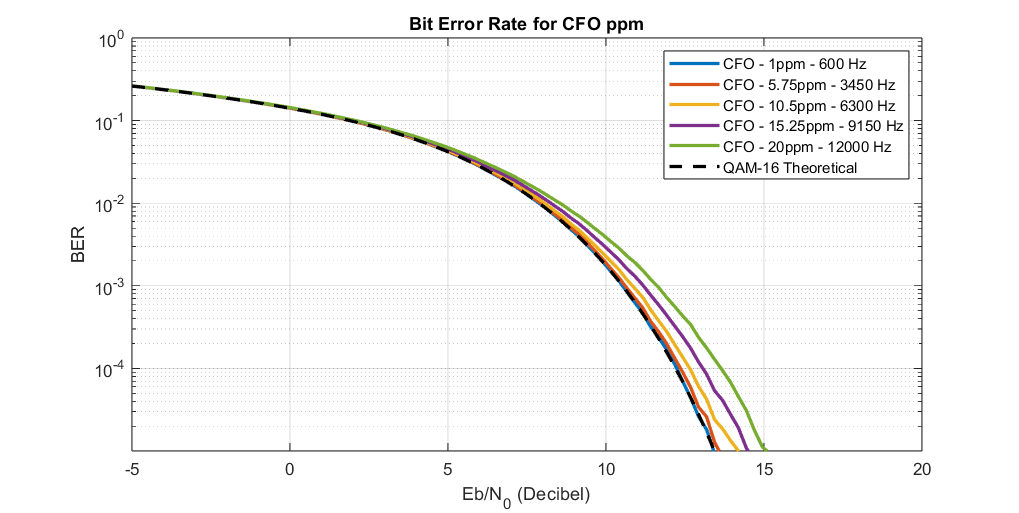
\includegraphics[width=0.8\textwidth]{CFO_ppm.png}
    \caption{BER with different CFO values}
    \label{fig:CFO_BER}
\end{figure}

Figure \ref{fig:CFO_const} shows the effect of CFO on the symbol constellation for QAM-16. It is here plotted without any noise and with parameters that allow us to see the line phase shift of the symbols. \\

\begin{figure}[H]
    \centering
    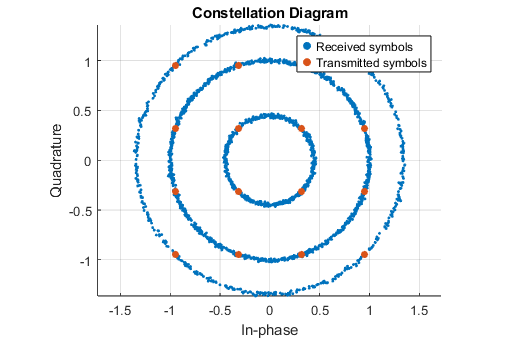
\includegraphics[width=0.8\textwidth]{constellation_CFO.png}
    \caption{Constellation before and after CFO}
    \label{fig:CFO_const}
\end{figure}

\subsection{Phase offset}
The same is done for the phase offset where the exponential is simply $e^{j\phi}$ where $\phi$ is chosen once at the begining of the simulation. \\

The effect of the phase offset is only visible on the constellation plot (figure \ref{fig:phaseOffsetConst}) where every point is rotated by a fixed angle (whereas CFO rotated the symbols linearly with time). \\

\begin{figure}[H]
    \centering
    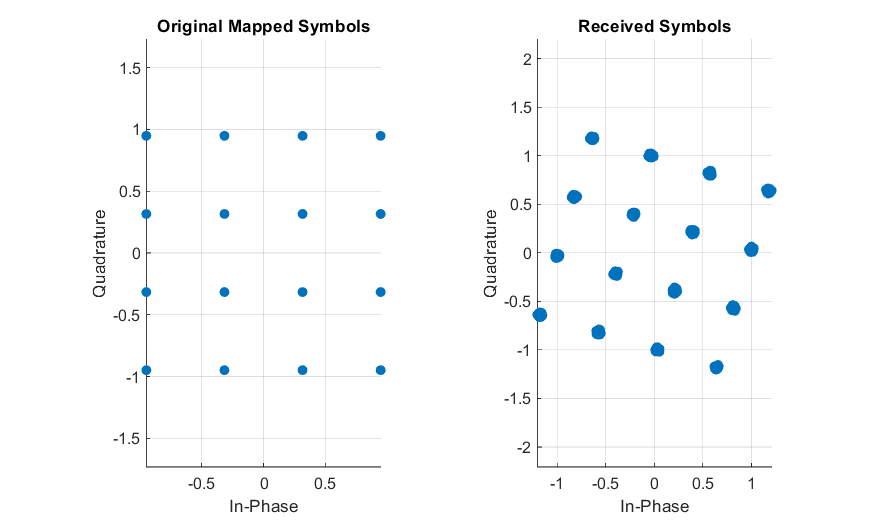
\includegraphics[width=0.8\textwidth]{constellation_carrier_offset.png}
    \caption{Constellation before and after phase offset}
    \label{fig:phaseOffsetConst}
\end{figure}

On a BER curve (figure \ref{fig:BER_PO}), the phase is not visible as from the errors originating from the phase offset are either on every symbol or on none and this is why the error does not depend anymore on $E_b/N_0$. \\

\begin{figure}[H]
    \centering
    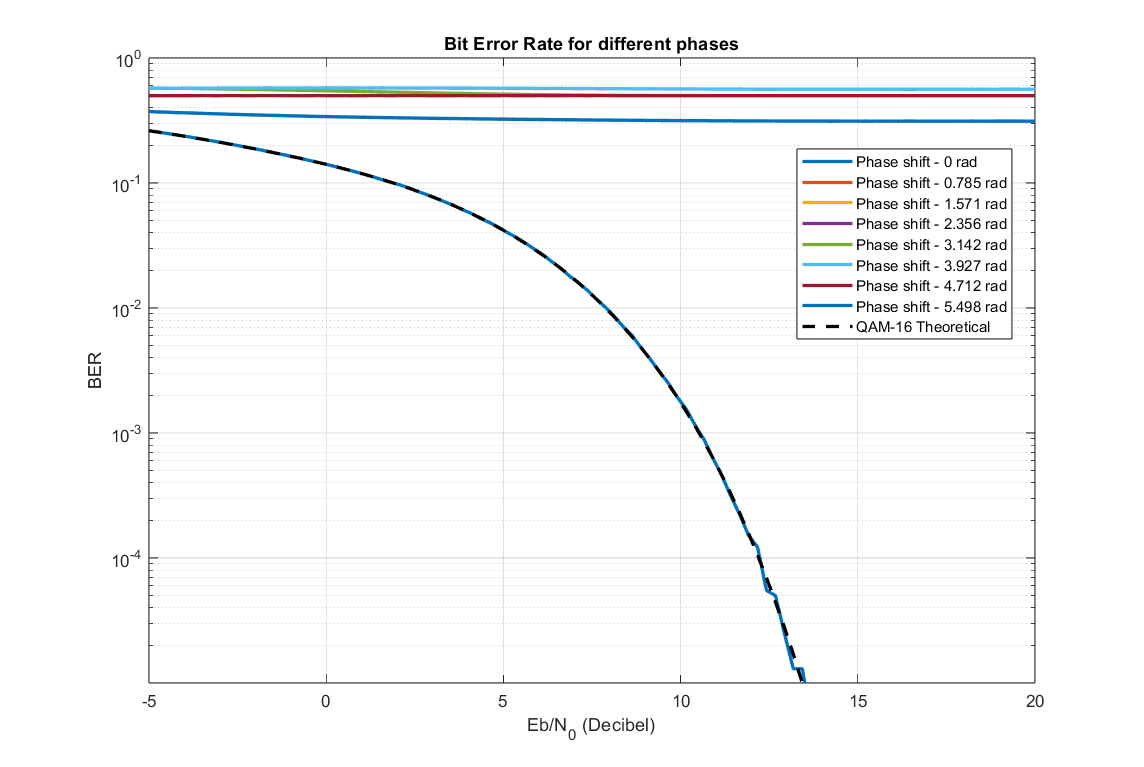
\includegraphics[width=0.8\textwidth]{BER_PO.png}
    \caption{BER with phase offset}
    \label{fig:BER_PO}
\end{figure}

\subsection{SFO}
The SFO is neglected in the simulation as it would need some interpolation and more complex computations. \\

\subsection{Time shift}
The time shift is implemented by simply shifting the samples in the array with an oversampling factor that is large enough. \\
A larger time shift will increase the BER as the samples will be taken at the wrong time. For sufficiently low values, it will still behave as a "classical" BER curve but from some point, there is just no more correlation between the measured sample and the received one and the BER tends to a $0.5$ line, as shown in figure \ref{fig:BER_TS}. \\

\begin{figure}[H]
    \centering
    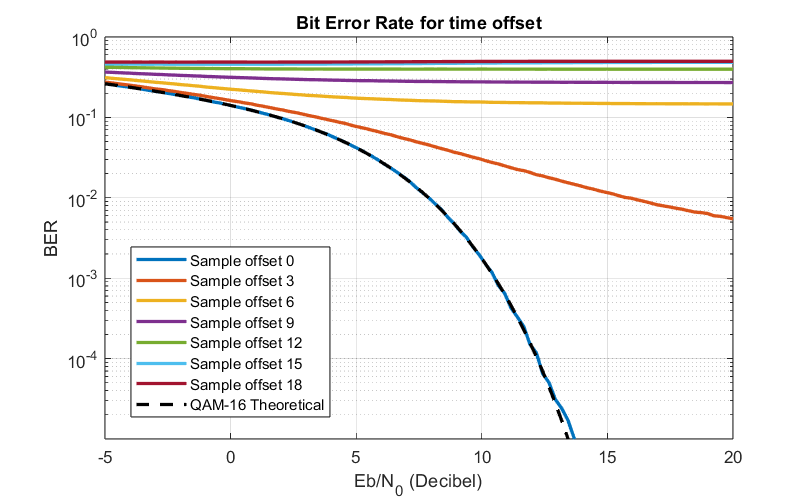
\includegraphics[width=0.8\textwidth]{BER_TS.png}
    \caption{BER with time shift}
    \label{fig:BER_TS}
\end{figure}

\section{Correction}




\chapter{Full channel simulation}

\section{Structure}
Now that every block of the transmission channel has been built and tested separately, the full channel can be simulated. It's structure is the following:
\begin{figure}[H]
    \centering
    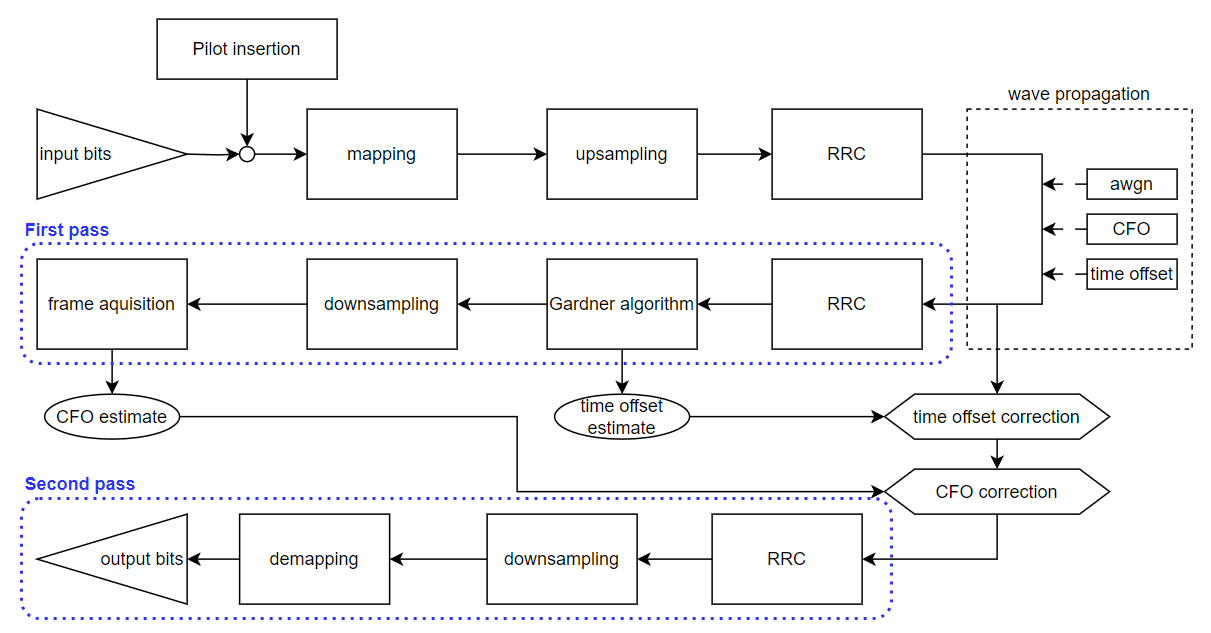
\includegraphics[width=0.8\textwidth]{pic/Full_channel.png}
    \caption{Full channel structure}
    \label{fig:full_channel}
\end{figure}

\section{Single pilot}
The following figure shows the error between the input and the output bits of the channel and the position of the pilot:
\begin{figure}[H]
    \centering
    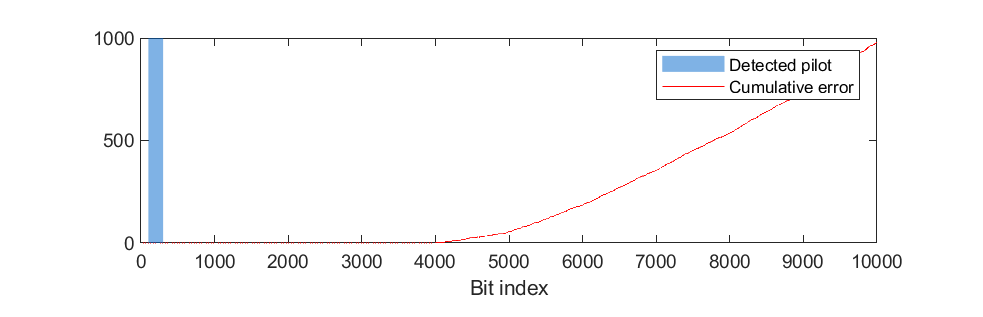
\includegraphics[width=0.8\textwidth]{pic/full_0.eps}
    \caption{Error between input and output bits for a single pilot ($N=50$, $K=12$)}
    \label{fig:full_0}
\end{figure}
As expected, the error is very low close at the beginning of the packet. This proves that the Gardner algorithm has successfully estimated the time offset and the CFO estimation was close to the real value. \\
Errors start to appear after $4000$ bits due to the linearly increasing phase added by the CFO. This simple example showed the importance of having multiple pilots in a packet.

\section{Multiple pilots}

As shown on figure \ref{fig:CFO_std_CFO_N}, the standard deviation of the CFO estimation is lowered for a longer pilot but it still remains different from zero. This means that multiple pilots should be sent in order to have a better estimation of the CFO. \\
This is what has been done in the following simulation. A total of $10$ pilots of $N=50$ bits have been sent in a packet of $10.000$ bits. The CFO is computed based on each pilot separately and the final estimation is the average of the individual estimations. The estimated CFO of the case in figure \ref{fig:full_1} is $3.098$ ppm for an actual value of $3$ ppm, which is quite close.\\
Because the channel is fully simulated, awgn is present and the $E_b/N_0$ is set to $10$ dB. \\
Once again, most of the errors are located closer to the end of the packet because the phase shift due to uncorrected CFO is linearly increasing with the bit index.

\begin{figure}[H]
    \centering
    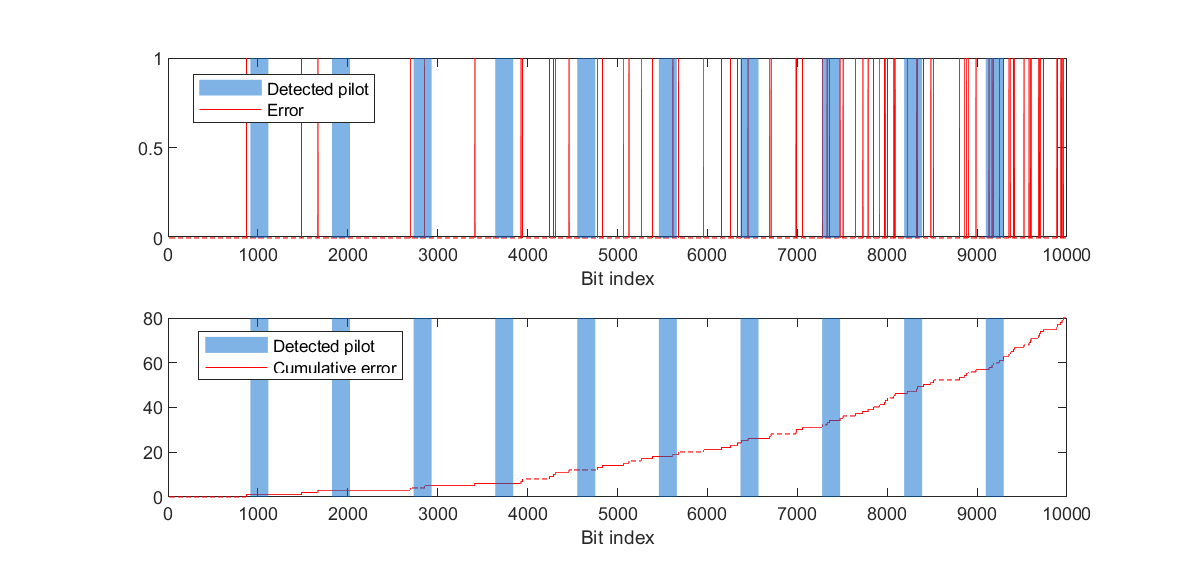
\includegraphics[width=0.8\textwidth]{pic/full_1.eps}
    \caption{Error between input and output bits for multiple pilots ($N=50$, $K=30$)}
    \label{fig:full_1}
\end{figure}

For this same case, the constellation diagrams of different signals are shown in figure \ref{fig:full_2}: 
\begin{itemize}
    \item The one in the top left corner is the input signal. 
    \item Below it, the output signal if no CFO compensation and no time shift corrector are applied. It is chaotic and no information can be retrieved from it.
    \item The top right corner shows the output signal after the Gardner algorithm has been applied. The time shift is corrected but the CFO is still present. The constellation is now made of 2 circles, which already shows that the modulation used is QAM-16. Those circles are the result of the CFO (as shown previously in figure \ref{fig:CFO_const})
    \item The bottom right corner shows the output signal after the Gardner algorithm and the CFO compensation have been applied. The points are now grouped around the initial constellation points. They are not perfectly aligned because the CFO estimation is not perfect and because of the noise added to the signal.
\end{itemize}

\begin{figure}[H]
    \centering
    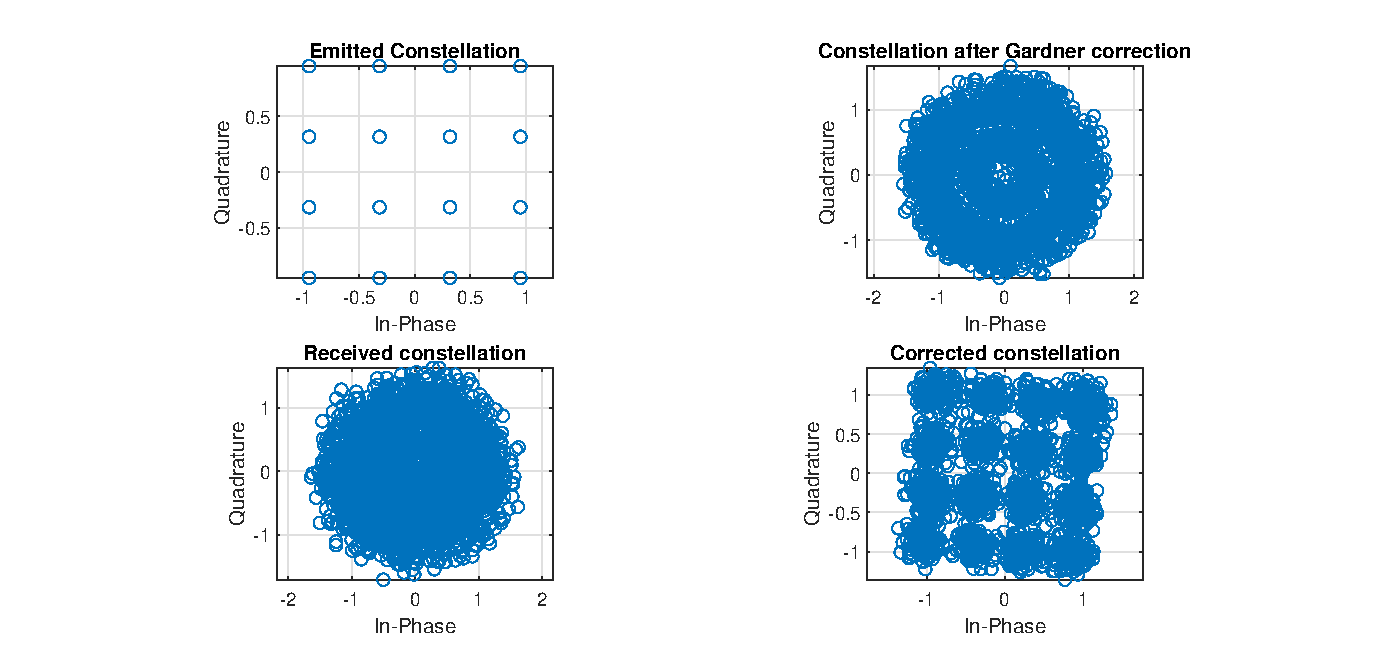
\includegraphics[width=0.8\textwidth]{pic/full_2.eps}
    \caption{Constellation diagrams for multiple pilots ($N=50$, $K=30$)}
    \label{fig:full_2}
\end{figure}

\chapter{Orange visit}

\subsection{Describe the architecture of the HFC network and its main components. Where
is the capacity bottleneck today?}

HFC stands for Hybrid Fiber Coaxial. It means that the network is made of both fiber optic and coaxial cables. The optic fiber is used between the headend and the \textit{nodes} and the coaxial cables are used from those nodes to the individual houses. \\
The coaxial part is the bottleneck but upgrading to fiber is very expensive and would need a cooperatin between the different operators.

\subsection{What will be the evolution of the HFC network in the coming years? What are the key technologies to make this happen?}

The \textit{nodes} discussed in the previous question will be shifted towards the houses and, after some time, the objective is to have a direct fiber connection from the headend to each house. This is done by splitting the light for downstream and a \textit{time division multiplexing} for upstream traffic. 

\subsection{Which are the typical incidents happening on Orange's network? Explain the procedure foreseen to cope with them.}

A tipical incident is a broken cable. It can happen due to civil works, weather conditions and so on. \\
If no signal can be sent through the line, the broken segment is idenified and the exact distance at which it broke is computed using the \textit{Optical Time Domain Reflectometer} (OTDR). It computes the time it takes for a light pulse to go through the fiber and come back (bounce due to unproper termination).\\
A technician is then sent to the location to solder the two broken fiber ends together and all of it happens in typically less than 8 hours.

\subsection{Describe the main Orange's data center in numbers (storage, in/out capacity, consumed power, area, maintenance...). How does it compare to others?}

Not much data was given about the data center. It consumes $1.5$ MW of power (which will increase to $3$ MW when the datacenter will be used at full capacity). The building is $3.000$ m$^2$ large and the data center moves $23$ TB of data every second. It also requires 2 technicians to be maintained. \\
It is complicated to compare it to other data centers because the data is not public.

%\printglossary

%\printglossary[type=\acronymtype]

%Bibliography
%\nocite{*}
%\printbibliography[type=article,title=Articles]

\end{document}	
